%
% $XORP: xorp/docs/libxipc/xrl_interfaces.tex,v 1.21 2006/08/02 00:59:43 pavlin Exp $
%

\documentclass[11pt]{article}

%\usepackage[dvips]{changebar}

\usepackage{subfigure}
\usepackage{fullpage}
\usepackage{setspace}
\usepackage{times}
\usepackage{latexsym}
\usepackage{epsfig}
\usepackage{graphicx}
\usepackage{xspace}
\usepackage{color}
\usepackage{amsmath}
\usepackage{rotating}
\usepackage{moreverb}
\usepackage{listings}
\usepackage{alltt}
\usepackage{stmaryrd}
%\usepackage[dvipdf]{graphics}
%\usepackage[dvips]{graphicx}
%\usepackage{xorp}

\definecolor{gray}{rgb}{0.5,0.5,0.5}
\newcommand{\etc}{\emph{etc.}\xspace}
\newcommand{\ie}{\emph{i.e.,}\xspace}
\newcommand{\eg}{\emph{e.g.,}\xspace}
%\newcommand{\comment}[1]{{\color{gray}[\textsf{#1}]}}
%\newcommand{\comment}[1]{}

% Changebar stuff
% \newenvironment{colorcode}{\color{blue}}{}
% \renewcommand{\cbstart}{\begin{colorcode}}
% \renewcommand{\cbend}{\end{colorcode}}

% \pagestyle{empty}

\begin{document}

\title{XRL Interfaces: Specifications and Tools \\
\vspace{1ex}
Version 1.3}
\author{ XORP Project					\\
	 International Computer Science Institute	\\
	 Berkeley, CA 94704, USA			\\
         {\it http://www.xorp.org/}			\\
	 {\it feedback@xorp.org}
}
\date{August 2, 2006}

\maketitle


%%%%%%%%%%%%%%%%%%%%%%%%%%%%%%%%%%%%%%%%%%%%%%%%%%%%%%%%%%%%%%%%%%%%%%%
%
% Local definitions
%
\newcommand{\clntgen}{{\sf clnt-gen}~}
\newcommand{\tgtgen}{{\sf tgt-gen}~}

% Configure listings
\lstloadlanguages{C++,C}
\lstset{
    tabsize=8
  , basicstyle=\ttfamily\small
  , commentstyle=\color{green}
  , flexiblecolumns=false
  , frame=TB
  , language=C++
  , stringstyle=\ttfamily
  , showstringspaces=false
}

%%%%%%%%%%%%%%%%%%%%%%%%%%%%%%%%%%%%%%%%%%%%%%%%%%%%%%%%%%%%%%%%%%%%%%%
\begin{abstract}

XORP Resource Locators are the XORP projects preferred means for
inter-process communication.  A description of the XRL's can be found
in \cite{xorp:xrl}.  This document describes an important aspect of the XRL
world: the specification of XRL Interfaces and Targets.  Following
these specifications this document then describes tools that generate
XRL marshalling and unmarshalling routines and assist in common case
XRL handling.

\end{abstract}

%%%%%%%%%%%%%%%%%%%%%%%%%%%%%%%%%%%%%%%%%%%%%%%%%%%%%%%%%%%%%%%%%%%%%%%
\section{Introduction}

Up until the interface specification language and tools described
here, only a low-level API was available for dispatching and handling
XRL requests.  The primary goal of the interface specification
language and tools is to make the common case XRL code less cumbersome
and more consistent.  In addition, the interface specification
language embeds versioning information which can be used to maintain
backwards compatibility as interface develop and minimize conflicts
following revisions.

%%%%%%%%%%%%%%%%%%%%%%%%%%%%%%%%%%%%%%%%%%%%%%%%%%%%%%%%%%%%%%%%%%%%%%%
\section{Terminology}

We define an \emph{XRL Target} as something that XRL requests can be
directed to in order to be executed.  Multiple XRL targets can
exist within a single process, though there will typically be one
target per process.  Each XRL Target has an associated name and a set
of IPC mechanisms that it supports.  At start-up each target registers
its name and IPC mechanisms with the Finder, so other processes are
able to direct requests to it.

We define an \emph{XRL Interface} to be a set of related methods that
an XRL Target would implement.  Each XRL Interface is uniquely
identified by a name and version number.  An XRL Target will nearly
always implement multiple interfaces and potentially multiple versions
of particular interface.  For instance, every XRL Target could
implement a process information interface that would return
information about the process hosting the target.  Each XRL Target
will implement interfaces specific to their field of operation: a
routing process would implement the ``routing process interface'' so
that the RIB process can make identity-agnostic XRL calls for tasks
like redistributing a route to another routing protocol.

We define an \emph{XRL Interface Client} to be a process that accesses
a particular XRL Interface.

These definitions are illustrated in figure \ref{fig:eg-interfaces}.

\begin{figure}
  \begin{center}
    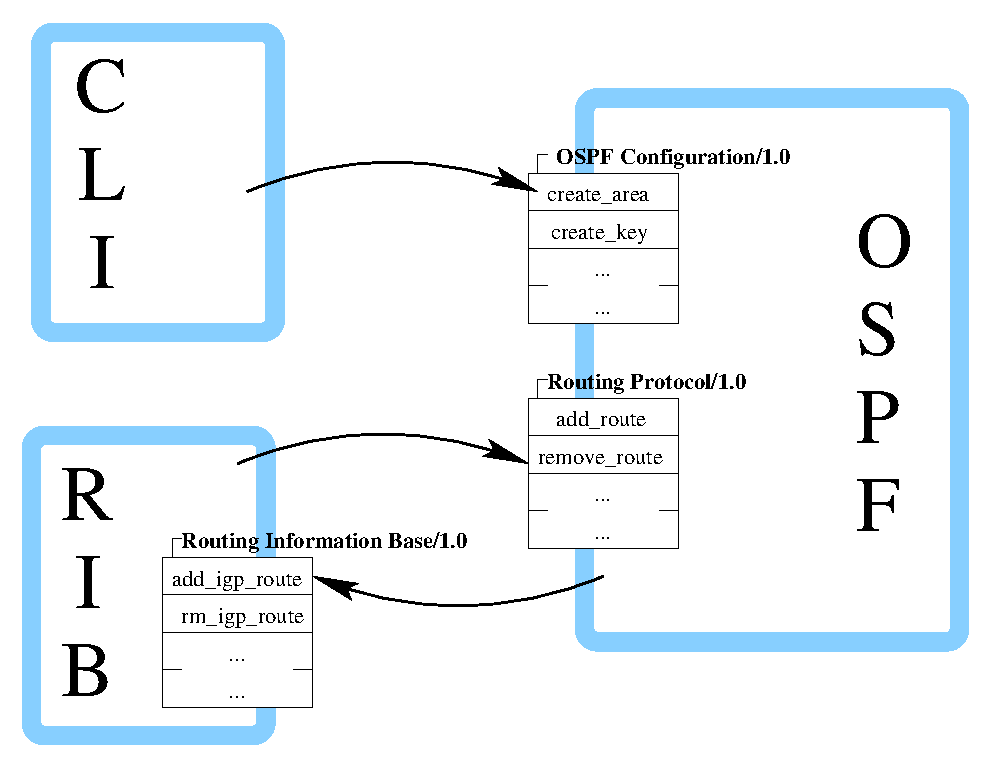
\includegraphics[width=0.75\textwidth]{figs/xrl_ifs}
  \end{center}
  \caption{Example XRL Targets and clients: OSPF, RIB, and CLI.
OSPF and RIB processes are XRL targets.  OSPF supports XRL interfaces
``OSPF Configuration/1.0'' and ``Routing Protocol/1.0'': the CLI is a
client of the ``OSPF Configuration/1.0'' interface and the RIB a client
of the ``Routing Protocol/1.0'' interface.  RIB supports XRL interface
``Routing Information Base/1.0'': the OSPF is a client of that interface.
}
  \label{fig:eg-interfaces}
\end{figure}

%%%%%%%%%%%%%%%%%%%%%%%%%%%%%%%%%%%%%%%%%%%%%%%%%%%%%%%%%%%%%%%%%%%%%%%
\section{Interface and Target Specifications}

%%%%%%%%%%%%%%%%%%%%%%%%%%%%%%%%%%%%%%%%%%%
\subsection{Interface Specifications}

An interface is declared using the \textbf{interface} keyword and a
set of XRL methods associated with it.

\smallskip
\noindent\framebox[\textwidth]{
   {\bf interface} $<${\it interface name}$>$/$<${\it interface version}$>$
   \{
     \dots {\it xrl method\ list} \dots
   \}
}

\smallskip Each item in the XRL Method list consists of a method name, its
dispatch arguments, and return arguments specified in the default XRL
text form.  An example of this is shown in listing \ref{lst:eg-interface}.

\lstinputlisting[%
  caption={Example Xrl Interface Specification%
    \label{lst:eg-interface}%
  }]{../../xrl/interfaces/test.xif}

Whitespace can be used to separate XRL Atoms in the description and
backslashes can be used to continue XRL descriptions across multiple
lines.  [NB This usage of spacing is not currently supported
elsewhere in the project - to be fixed.]

C-style comments are valid anywhere with interface specification files
and kdoc comments can be used to describe the XRL, its arguments, and
return values.  Each kdoc comment is associated with the next XRL
found in a specification file.  All kdoc tags are valid with the
exception of \textbf{@return} which is used by kdoc to describe C/C++
single return values (for XRL's return values should be document with
\textbf{@param} since they are named and groups of values can be
returned).

By convention, XRL Interfaces are specified in \texttt{.xif} files and these
are located in the \\
\texttt{xorp/xrl/interfaces} directory.

%%%%%%%%%%%%%%%%%%%%%%%%%%%%%%%%%%%%%%%%%%%
\subsection{Target Specifications}

XRL Targets are declared in \textit{.tgt} files using:

\smallskip
\noindent\framebox[\textwidth]{
 \textbf{target} $<target\ name>$ \textbf{implements}
  $<${\it interface}$>$ [, {$<${\it interface}$>$ \dots } ]
}

\smallskip Target specification files use the standard C include
primitive to include the appropriate interface specifications.  An
example is shown in listing \ref{lst:eg-target} and further examples
can be found in the \texttt{xorp/xrl/targets} directory.

\lstinputlisting[%
  caption={Example XRL Target
  specification.\label{lst:eg-target}}]%
{../../xrl/targets/test.tgt}

%%%%%%%%%%%%%%%%%%%%%%%%%%%%%%%%%%%%%%%%%%%%%%%%%%%%%%%%%%%%%%%%%%%%%%%
\section{Tools}

We use XRL Interface and XRL Target specifications to generate code
that takes some of the tedium out of writing XRL related code.  We
have written two scripts: \clntgen and \tgtgen that
generate C++ header files and libraries and also produce a list of
XRL's for each XRL Target.

%%%%%%%%%%%%%%%%%%%%%%%%%%%%%%%%%%%%%%%%%%%
\subsection{\clntgen : XRL Interface Client Generator}

\clntgen parses Xrl Interface specifications and generates a header
and related library source file to simplify invoking the XRL's of that
interface.  Each XRL Interface specification generates an XRL
Interface Client C++ class.  The generated C++ class has a send method
for each XRL in the XRL interface specification and takes care of
argument marshalling when the XRL is dispatched and when it returns.

A fragment of generated code is shown in listing \ref{lst:client-code}.
This code is generated from the Xrl Interface presented in listing
\ref{lst:eg-interface}.  The Xrl Interface Client C++ has a constructor
that takes a XrlRouter object that holds the necessary state to
correlate the XRLs being called with the return values.  Each XRL
specified in the XRL Interface has a send method.  The send method
takes the name of Xrl Target, the native C++/XORP arguments to be
passed as XRL arguments, and a callback argument to be invoked when
the XRL returns.

The type of the XRL callback is determined by the return type
specification of the XRL.  Since the syntax for the callback is awkward,
a typedef is used in the class method.  The relevant typedef appears
immediately before each send method.  When called, the first callback
argument of the callback is an {\tt XrlError} object.  If the value is
{\tt XrlError::OKAY()} then return values from the XRL will be pointed
to by the following arguments (\eg, const string* for string argument).
Otherwise, the return value pointers will be {\tt NULL} since there is
no data available for return values when errors occur.

The interested reader should refer to the directory {\tt xorp/xrl/tests/}
for examples using the client interface.

%\newpage
\begin{lstlisting}[caption={ Fragment of a C++ XRL Client. %
                                     \label{lst:client-code} } ]{}

class XrlTestV1p0Client {
public:
    XrlTestV1p0Client(XrlRouter* r) : _router(r) {}
    virtual ~XrlTestV1p0Client() {}

    /* ... */

    typedef XorpCallback2<void, const XrlError&, const string*>::RefPtr CB3;
    /**
     *  Send Xrl intended to:
     *
     *  Get greeting.
     *
     *  @param dst_xrl_target_name the Xrl target name of the destination.
     *
     *  @param greeting_num index of greeting.
     */
    void send_get_greeting(
        const char*     dst_xrl_target_name,
        const int32_t&  greeting_num,
        const CB3&      cb
    );

    /* ... */
};
\end{lstlisting}

%%%%%%%%%%%%%%%%%%%%%%%%%%%%%%%%%%%%%%%%%%%
\subsection{\tgtgen : XRL Target Generator}

\tgtgen takes an XRL target specification and generates list of XRL's
supported by the target and a class to be sub-classed that takes care
of argument marshalling and unmarshalling and sanity checks.

The XRL's for the {\tt test/1.0} that was target presented in listing
\ref{lst:eg-target} are shown in listing \ref{lst:eg-xrls}.  Notice
that the name of each XRL has the interface and version that it
belongs to prepended.  This is the mechanism used to support the
concept of interfaces and to support versioning.

\lstinputlisting[%
  caption={Example XRL list generated from Xrl Target specification. %
           \label{lst:eg-xrls}}, language=C, basicstyle=\ttfamily\scriptsize,float]%
  {../../xrl/targets/test.xrls}

As far as the generated base class is concerned, it implements a set
of pure-virtual Xrl handler methods each of which is associated with
handling a specific XRL.  The implementor derives from the base class,
implementing the pure-virtual methods.  When an XRL request is
received, it will be forwarded to the derived class's implementation
handler method.  The base class takes care of marshalling and
unmarshalling Xrl arguments and error handling.

The design to derive a class to implement the handler functions was,
in part, taken to encourage (force) people to implement handlers for
all the XRL's specified for the XRL Target.  In addition, implementors
can add whatever state they require in dispatching XRL's to the
handler class, ie pointers or references to data structures.

An example of a generated target header is shown in listing
\ref{lst:eg-tgt-header}.  Notice that the input Xrl arguments are
const reference arguments to the C++ method, and the Xrl return
arguments are just reference arguments.

\newpage
\lstinputlisting[caption={Example Xrl Target C++ Base Class %
                          \label{lst:eg-tgt-header}}, basicstyle=\ttfamily\scriptsize]%
                {../../xrl/targets/test_base.hh}

%%%%%%%%%%%%%%%%%%%%%%%%%%%%%%%%%%%%%%%%%%%%%%%%%%%%%%%%%%%%%%%%%%%%%%%
%     APPENDIX
%%%%%%%%%%%%%%%%%%%%%%%%%%%%%%%%%%%%%%%%%%%%%%%%%%%%%%%%%%%%%%%%%%%%%%%
\appendix
\section{Modification History}

\begin{itemize}

  \item December 11, 2002: Initial version 0.1 completed.

  \item March 10, 2003: Minor changes.
  Updated the version to 0.2, and the date.

  \item June 9, 2003: Updated the version to 0.3, and the date.

  \item August 28, 2003: Updated the version to 0.4, and the date.

  \item November 6, 2003: Updated the version to 0.5, and the date.

  \item July 8, 2004: Updated the version to 1.0, and the date.

  \item April 13, 2005: Updated the version to 1.1, and the date.

  \item March 8, 2006: Updated the version to 1.2, and the date.

  \item August 2, 2006: Updated to match XORP release 1.3: fixed sample
  XRL-related code to match the current code.
  Added ``Modification History'' appendix.

\end{itemize}

%%%%%%%%%%%%%%%%%%%%%%%%%%%%%%%%%%%%%%%%%%%%%%%%%%%%%%%%%%%%%%%%%%%%%%%
%     BIBLIOGRAPHY
%%%%%%%%%%%%%%%%%%%%%%%%%%%%%%%%%%%%%%%%%%%%%%%%%%%%%%%%%%%%%%%%%%%%%%%
\bibliography{../tex/xorp}
\bibliographystyle{plain}

%%%%%%%%%%%%%%%%%%%%%%%%%%%%%%%%%%%%%%%%%%%%%%%%%%%%%%%%%%%%%%%%%%%%%%%
\end{document}
